\documentclass{standalone}
\usepackage{tikz}
\usetikzlibrary{calc}
\begin{document}

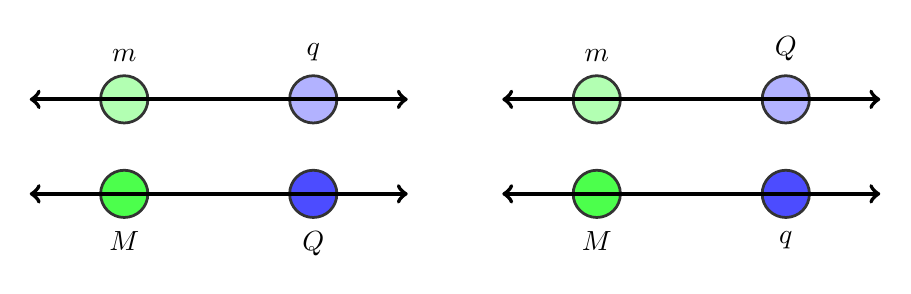
\begin{tikzpicture}[scale=1.2]
% \draw[step=0.5cm,gray!50,very thin] (-6,-6) grid (6,6);
% \draw[->,thin] (0,-6) -- (0,6);
% \draw[->,thin] (-6,0) -- (6,0);
% \draw (0,0) node[below] {$0$};
% \foreach \j in {-6, -5, ..., -1, 1, 2, ..., 6} {
%   \draw (\j,0) node[below=0.1]{\j};
%   \draw (0,\j) node[right=0.1]{\j};
% }

\coordinate (m) at (1,3);
\coordinate (q) at (3,3);
\coordinate (M) at (1,2);
\coordinate (Q) at (3,2);

\filldraw[fill=green!30, draw=black!80, line width=1pt] (m) circle (0.25cm) node[above=0.35cm] {$m$};
\filldraw[fill=blue!30, draw=black!80, line width=1pt] (q) circle (0.25cm) node[above=0.35cm] {$q$};
\filldraw[fill=green!70, draw=black!80, line width=1pt] (M) circle (0.25cm) node[below=0.35cm] {$M$};
\filldraw[fill=blue!70, draw=black!80, line width=1pt] (Q) circle (0.25cm) node[below=0.35cm] {$Q$};
\draw[<->,line width=1.5pt] ($(m)-(1,0)$)   -- ($(q)+(1,0)$);
\draw[<->,line width=1.5pt] ($(M)-(1,0)$)   -- ($(Q)+(1,0)$);


\coordinate (m) at (6,3);
\coordinate (Q) at (8,3);
\coordinate (M) at (6,2);
\coordinate (q) at (8,2);

\filldraw[fill=green!30, draw=black!80, line width=1pt] (m) circle (0.25cm) node[above=0.35cm] {$m$};
\filldraw[fill=blue!30, draw=black!80, line width=1pt] (Q) circle (0.25cm) node[above=0.35cm] {$Q$};
\filldraw[fill=green!70, draw=black!80, line width=1pt] (M) circle (0.25cm) node[below=0.35cm] {$M$};
\filldraw[fill=blue!70, draw=black!80, line width=1pt] (q) circle (0.25cm) node[below=0.35cm] {$q$};
\draw[<->,line width=1.5pt] ($(m)-(1,0)$)   -- ($(Q)+(1,0)$);
\draw[<->,line width=1.5pt] ($(M)-(1,0)$)   -- ($(q)+(1,0)$);

\end{tikzpicture}

\end{document}